% !TeX root = main.tex
\chapter{Introduction}
To survive in an ecosystem organisms need to adapt to the specific abiotic and biotic factors around them. This is particularly important for plants since they can not change their habitat during their lifespan. The necessary adaptation can occur on different levels of the organisms, starting from the adaptation of protein function to modifications in cell functions and whole tissue properties. In all of these cases the fundamental process driving adaptation is the modification of the genetic material: DNA (Griffith, 1928\cite{Griffith1928}).\\
Modifications on DNA level are called mutations and can be distributed throughout the genome. Here we will constrict our analysis to mutations which occur in coding regions of the genome although they can be distributed also in intergenic regions. A simple explanation is based on the outcome of mutations. Mutations in the coding regions of the genome can have a direct impact on the amino acid sequence and therefore influence the protein functionality, which is described in the following. But mutations that occur in intergenic regions do have indirect impact on many processes in the cell by mainly influencing the gene regulation. In our further analysis we are not interested in these regulatory changes rather we are interested in how changes in the coding regions affect adaptation.\\
Mutations can be classified into four different groups. The first group of mutations to consider is the point mutation since it is concerning just one single base pair (bp). Since these mutations only change a single point in the DNA sequence they will directly result in changes to the transcribed mRNA. Another class of mutations are insertions. Here a new sequence is inserted into the original DNA sequence which results in its elongation. Insertions can have a variety of lengths from one single base pair to a few hundred base pairs and even longer sequences. The contrasting class of insertions are deletions, which lead to a reduction of a number of base pairs. They can likewise result in a variety of lengths of the mutated DNA strand. The fourth and last category of mutations are duplications. As implied by the name, regions of the DNA get duplicated and inserted at a different position. The regions can be copied abnormally one or even more times.\\
The impact of mutations on the biochemical processes inside a cell and an organisms phenotype is determined by its influence on protein creation. In this process the DNA first gets transcribed into mRNA, a step that is not affected by the mutations. The mRNA is translated into proteins in the following step. Here the mutations have a direct impact as each triplet base pair (codon) gets translated into a specific amino acid, which can change due to the mutation in the DNA as postulated by Gamow\cite{crick1988}.The specific mapping between amino acids and these codons was deciphered by \textcite{Nirenberg1965}. \autoref{fig:Codons} a) shows how each triplet codon is translated into a specific amino acid or indicates a stop codon, providing the universal genetic code that links RNA sequences and proteins. The fact that only 20 amino acids are matched with $4^3 = 64$ unique codons led \textcite{Lagerkvist1978} to the insight that this code is degenerated. This means that a single codon is not directly linked to a single amino acid, but that multiple codons are translated to the same amino acid.\\
Based on this translation table we can now understand that mutations can have different effects on the resulting protein. In most cases, insertions or deletions result in a shift of the reading frame and therefore change the sequence of amino acids in a wide range extending the region of the mutation. While point mutations only influence a single codon, they can still have different effects on the translated amino acid and therefore on the functionality of the resulting protein. We distinguish three possible outcomes of such a mutation on protein level: (i) A synonymous mutation, where the protein is not changed at all. Here a base pair changes but the translated codons provoke the same amino acid. An example for a synonymous mutation is provided in \autoref{fig:Codons} b). (ii) Non-synonymous mutations resulting in the exchange of the amino acid type as shown in \autoref{fig:Codons} c). Predicting the severity of non-synonymous mutations is hard to do without further analysis since it depends on many circumstances like the location of the changed amino acid with respect to the catalytic region of the protein or the specific amino acids involved in the exchange. Therefore these mutations vary in their significance between almost unnoticeable and making the protein non-functional. (iii) Premature stop codons: This kind of mutation changes a usual codon to a stop codon as presented in \autoref{fig:Codons} d). This will almost always result in drastic changes to the protein functionality since the resulting protein is truncated. Due to this they represent one of the most interesting kind of mutations for understanding adaptation in plants. Premature stop codons can be recognized on the DNA level and will directly impact the function of the truncated protein in almost every case.\\
\begin{figure}[tb]
    \centering
    \begin{minipage}[h]{0.9\textwidth}
      \centering
      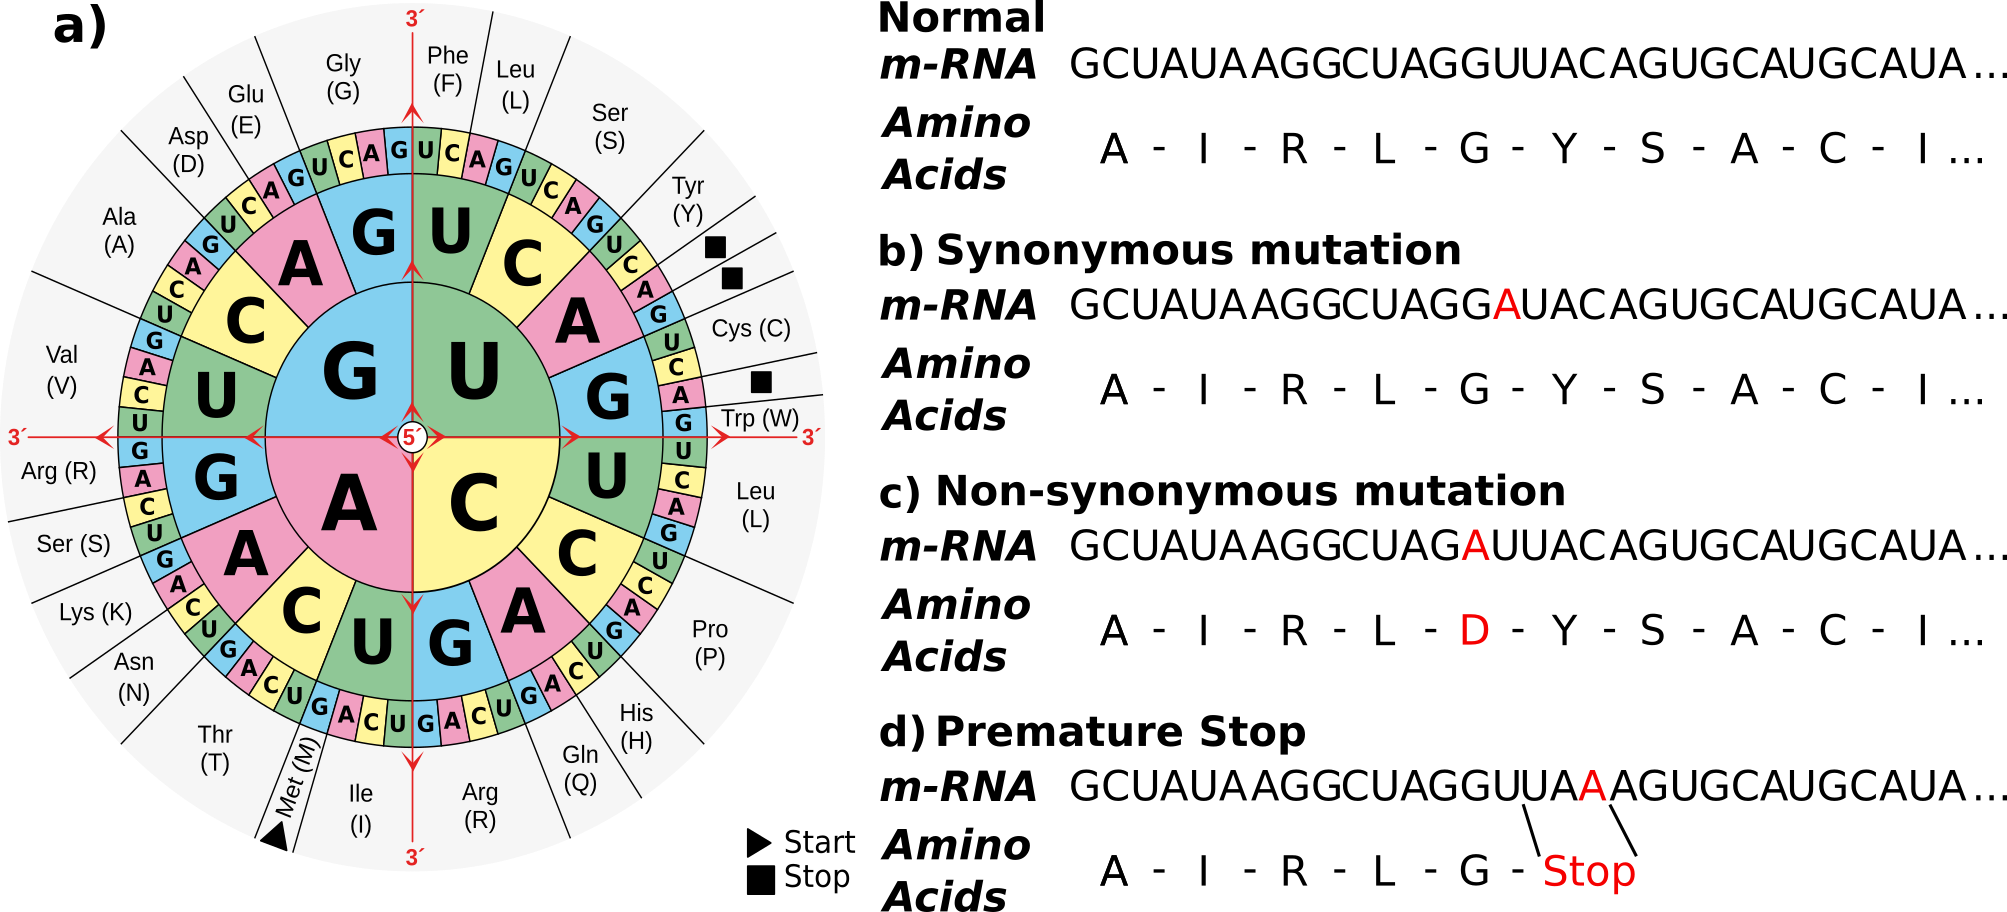
\includegraphics[width=1\textwidth]{images/Mutations.png}
      \caption[Schematic representation of point mutation classes]{\textbf{Schematic representation of point mutation classes}\\
      a) The genetic code (image taken from \textcite{bresch2013}); b) An examplary representation of a synonymous mutation, which affects the mRNA but not the amino acid sequence. c) Example of a non-synonymous mutation. The change of a single base pair in the mRNA sequence leads to an exchange of the amino acid type. d) Example of a premature stop codon mutation. Induced by the exchange of a single base pair a premature stop codon appears and stops the amino acid sequence.}
     \label{fig:Codons}
    \end{minipage}
  \end{figure}
Driven by our interest in adaptation over an evolutionary timescale we study mutations on a population scale in this thesis. Point mutations which occur on population scale are called single-nucleotide polymorphisms (SNPs). Each SNP defines a difference at a  specific position in the genome that appears in the population. This way we can distinguish individuals which have the reference allele at this position (no point mutation) from individuals which have the alternative allele (a change of the base pair). These SNPs are distributed throughout the whole genome and can be used to analyse patterns of mutations statistically and correlate them to phenotypic effects. \\
Until recently, evolutionary theory was working with the assumption that all types of mutations referenced above occur randomly throughout the genome initially and that evolutionary selection only influences their presence in a populations genetic pool after their occurrence (Futuyma 1986\cite{futuyma1986}). From this starting point one can deduce the natural selection removes fatal modifications from the genetic pool and generically influences the occurrence mutations depending on their severity. This also implies that mutations with neutral significance like synonymous mutations are not shaped by the selection force. On the other side positive impact is reinforced by the selection force, leading to an accumulation of these mutations in the genetic pool (Darwin 1909 \cite{darwin1909}).\\
By summarizing these described processes we can draw conclusions of expected adaptation processes in organisms. Combining that mutations act as a fundamental force of evolution and that natural selection is shaping the population we can get an understanding of how adaptation shapes an individual organisms. Restricting our view to mutations of premature stop codon type and considering the adaptation of an organisms to abiotic and biotic factors as a complex gene-regulatory networks that is regulated, we can hypothesize the effects of mutations on these networks. Since the occurrence of premature stop codons is directly resulting in a loss of function of the affected protein one can assume that evolutionary selection force stabilizes the surrounding gene regulatory network by maintaining the diversion of this networks. Practically this means that if a protein is knocked out by a premature stop codon the pathways surrounding this damaged one are getting more important and you expect them to be under a high conservation force by evolutionary selection. The selection should prevent a accumulation of premature stop codons in the rest of the gene regulatory network to conserve the original functionality of a network as best as possible.\\
In this thesis we want to study the attributes and occurrence of these premature stop codons in a population of \textit{Arabidopsis thaliana}. We characterize how the natural selection is shaping population structures through generating loss-of-function variants and how they affect the adaptation process of organisms. We accomplish this by following a bioinformatical approach i.e. by applying data analysis and statistical algorithms on different genomic data in order to identify evolutionary patterns. 